% Calendar-wheel figure — distribution of PlantCLEF 2026 test quadrats
% by month of observation. Radial bar length is proportional to the
% number of quadrats observed in that month.
%
% Counts (from the paper text):
%   April + May + June     607  (aggregate; we distribute uniformly here)
%   July                   517  (exact)
%   August                 668  (exact)
%   the seven other months 313  (residual; distributed uniformly ≈ 45/mo)
%   total                  2105 quadrats
%
% The wheel is a temporal analogue of a geographic map: each sector is
% a month of the year, and bar length shows how many test quadrats fall
% in that month. The visually obvious summer over-representation is the
% load-bearing observation motivating the seasonal phenology pivot.
%
% Required host preamble:
%   \usepackage{tikz}

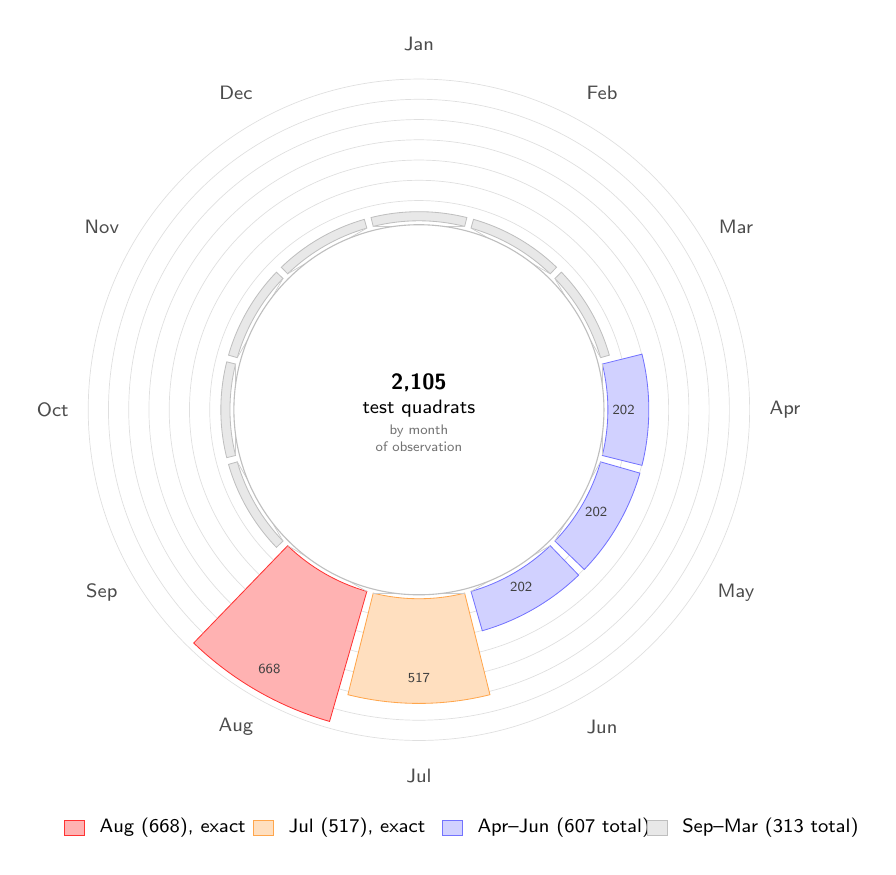
\begin{tikzpicture}[
  font=\sffamily\footnotesize,
]

% Geometry
\def\R{2.4}            % inner radius of the dial
\def\Router{4.2}       % outermost reachable radius (Aug peak)
\def\bartick{0.04}     % minor radial gridline thickness

% Convert a quadrat-count into a radius
% Aug (668) → \Router; counts scale linearly.
% Using a function-of-text would need pgfmath — we just precompute below.

% ── Radial gridlines (every 100 quadrats) ───────────────────────────────
\foreach \c/\ann in {100/, 200/, 300/, 400/, 500/, 600/, 700/} {
  \pgfmathsetmacro\rr{\R + (\Router-\R) * \c / 700}
  \draw[gray!25, line width=0.25pt] (0,0) circle (\rr);
}

% ── 12 month sectors with radial bars ───────────────────────────────────
% Each entry: month-index, label, count, fill colour, edge colour
\foreach \i/\lbl/\cnt/\fc/\sc in {
   1/Jan/45/gray!18/gray!50,
   2/Feb/45/gray!18/gray!50,
   3/Mar/45/gray!18/gray!50,
   4/Apr/202/blue!18/blue!55,
   5/May/202/blue!18/blue!55,
   6/Jun/202/blue!18/blue!55,
   7/Jul/517/orange!25/orange!70,
   8/Aug/668/red!30/red!80,
   9/Sep/45/gray!18/gray!50,
  10/Oct/45/gray!18/gray!50,
  11/Nov/45/gray!18/gray!50,
  12/Dec/45/gray!18/gray!50%
} {
  % Polar geometry: Jan is at the top (90°), then go clockwise.
  \pgfmathsetmacro\thetaStart{90 - (\i-1)*30 - 14}
  \pgfmathsetmacro\thetaEnd{90 - (\i-1)*30 + 14}
  \pgfmathsetmacro\thetaMid{90 - (\i-1)*30}
  \pgfmathsetmacro\rr{\R + (\Router-\R) * \cnt / 700}

  % Filled wedge (pie slice from inner radius to count radius).
  \filldraw[fill=\fc, draw=\sc, line width=0.3pt]
    (\thetaStart:\R) arc (\thetaStart:\thetaEnd:\R)
      -- (\thetaEnd:\rr) arc (\thetaEnd:\thetaStart:\rr) -- cycle;

  % Tiny outline of the wedge boundary at the inner radius (helps eye).
  \draw[gray!40, line width=0.25pt]
    (\thetaStart:\R) -- (\thetaEnd:\R);

  % Month label, placed just outside the maximum possible radius.
  \node[font=\sffamily\scriptsize, text=black!70]
    at (\thetaMid:\Router+0.45) {\lbl};

  % Count label inside the wedge, only when count > 100.
  \ifnum\cnt>100
    \node[font=\sffamily\tiny, text=black!75]
      at (\thetaMid:\rr-0.32) {\cnt};
  \fi
}

% ── Inner cap with total ────────────────────────────────────────────────
\filldraw[fill=white, draw=gray!50, line width=0.4pt] (0,0) circle (\R-0.05);
\node[align=center, font=\sffamily\footnotesize] at (0, 0.18)
  {\textbf{2{,}105}\\[-1pt]
   {\scriptsize test quadrats}};
\node[align=center, font=\sffamily\tiny, text=black!55] at (0, -0.36)
  {by month\\ of observation};

% ── Horizontal legend strip below the wheel ─────────────────────────────
% Placed at world y = -5.4 — well below the lowest wheel label (Aug at
% y ≈ -4.65) so there's no risk of bumping into any of the month
% annotations around the perimeter.
\begin{scope}[shift={(-4.5, -5.4)}]
  % Each entry is one swatch + label group; entries are spaced 2.4 apart.
  % Entry 1: Aug
  \draw[fill=red!30, draw=red!80, line width=0.3pt] (0, 0) rectangle ++(0.25, 0.18);
  \node[anchor=west, font=\sffamily\scriptsize] at (0.32, 0.09)
    {Aug (668), exact};

  % Entry 2: Jul
  \draw[fill=orange!25, draw=orange!70, line width=0.3pt] (2.4, 0) rectangle ++(0.25, 0.18);
  \node[anchor=west, font=\sffamily\scriptsize] at (2.72, 0.09)
    {Jul (517), exact};

  % Entry 3: Apr–Jun
  \draw[fill=blue!18, draw=blue!55, line width=0.3pt] (4.8, 0) rectangle ++(0.25, 0.18);
  \node[anchor=west, font=\sffamily\scriptsize] at (5.12, 0.09)
    {Apr--Jun (607 total)};

  % Entry 4: Sep–Mar
  \draw[fill=gray!18, draw=gray!50, line width=0.3pt] (7.4, 0) rectangle ++(0.25, 0.18);
  \node[anchor=west, font=\sffamily\scriptsize] at (7.72, 0.09)
    {Sep--Mar (313 total)};
\end{scope}

\end{tikzpicture}
